\documentclass[../main]{subfiles}
\begin{document}
\section{Mecánica de una partícula}
La mecánica de la partícula está regida por la \textit{Segunda Ley de Newton del Movimiento}, la cual establece que existen sistemas de referencia en los cuales el movimiento de la partícula esta descrita por la ecuación diferencial:
    \begin{align}
    \Vec{F}=\dv{}{t}\left(m\Vec{v}\right)=\dot{\vec{p}}
    \label{eq1}
    \end{align}
Donde $\vec{p}$ es la cantidad de movimiento de una partícula, la cual por definición es:
    \begin{equation}
	    \vec{p}=m\vec{v}
	    \label{eq2}
    \end{equation}
Por el \textbf{Teorema de conservación de la cantidad de movimiento de una partícula}: Si la fuerza resultante $\vec{F}_T$ es nula, tendremos que $\dot{\vec{p}}=0$ y se conservara la cantidad de movimiento $\vec{p}$.

\subsection*{Momento Cinético}
El momento cinético de la partícula respecto a un punto $O$ se presenta por $\vec{L}$ y se define como:
	\begin{equation}
	    \vec{L}=\vec{r}\times \vec{p}
	    \label{eq3}
	\end{equation}
donde $\vec{r}$ es el vector posición que va desde el punto $O$ hasta la partícula.

\subsection*{Momento de una Fuerza}
Definimos ahora el momento de una fuerza respecto a un punto $O$ de la forma:
	\begin{equation}
	    \vec{N}=\vec{r}\times \vec{F}
	    \label{eq4}
	\end{equation}
Utilizando la ecuación \eqref{eq1} para $\vec{N}$, y utilizando la \textit{identidad vectorial} obtenemos:
	\begin{equation}
	    \vec{N}=\vec{r}\times \dfrac{d}{dt}(m\vec{v})+\vec{v}\times m\vec{v}=\dfrac{d}{dt}(\vec{r}\times m\vec{v})
	    \label{eq5}
	\end{equation}
Donde de la ecuación \eqref{eq5} obtenemos la siguiente relación:
    \begin{equation}
        \vec{N}=\dfrac{\text{d}\vec{L}}{\text{d}t}
        \label{eq6}
    \end{equation}
Notamos que tanto $\vec{N}$ como $\vec{L}$ dependen del punto $O$ respecto al cual se toman los momentos. \\
Al igual que en la ecuación \eqref{eq1}, la ecuación \eqref{eq6} para el momento nos da el \textbf{Teorema de conservación del momento cinético de una partícula}: Si el momento resultante $\vec{N}$ es nulo, entonces $\dot{\vec{L}}=0$, y se conserva el momento cinético.

    \vspace{0.2cm}
    
Consideremos ahora el trabajo que se efectúa por la fuerza exterior $\vec{F}$ sobre una partícula cuando va del punto $1$ al punto $2$:
    \begin{equation}
        W_{12}=\int_1^2 \vec{F} \cdot \text{d} \vec{s}=m \int \dfrac{\text{d}\vec{v}}{\text{d}t}\cdot \vec{v} \text{d}t=\dfrac{m}{2}\int_1^2 \dfrac{\text{d}}{\text{d}t}(v^2) \text{d}t=\dfrac{m}{2}\left( v_2^2-v_1^2\right)
        \label{eq7}
    \end{equation}
La magnitud $\dfrac{1}{2}mv^2$ es la energía cinética de la partícula y se representa por $T$, con lo que el trabajo es igual a la variación de la energía cinética (\textbf{Teorema del Trabajo y la energía}):
    \begin{equation}
        W_{12}=T_2-T_1
        \label{eq8}
    \end{equation}
La independencia de $W_{12}$ del camino particular seguido implica que el trabajo efectuado a lo largo del circuito cerrado sea nulo, de la forma:
    \begin{equation}
        \oint \vec{F} \cdot \text{d}\vec{s}=0
        \label{eq9}
    \end{equation}
Para que $W_{12}$ sea independiente del camino físico seguido por la partícula es condición necesaria y suficiente que $\vec{F}$ sea el gradiente de una cierta función escalar de la posición:
    \begin{equation}
        \vec{F}=-\vec{\nabla} V(\vec{r})
        \label{eq10}
    \end{equation}
Si $W_{12}$ es independiente del camino de integración entre los extremos $1$ y $2$, se podría considerar que $W_{12}$ es la variación de una magnitud que sólo depende de la posición de los puntos extremos. Esta magnitud la podemos representar por $-V$ de la forma que:
    \begin{equation*}
        \vec{F}\cdot \text{d}\vec{s}=-\text{d}V
    \end{equation*}
o también de la forma:
    \begin{equation*}
        \vec{F}_s=-\dfrac{\partial V}{\partial s}
    \end{equation*}
En el caso de un sistema conservativo el trabajo efectuado por las fuerzas es:
    \begin{equation}
        W_{12}=\int_1^2 \vec{F} \cdot \text{d}\vec{s}=-\int \vec{\nabla} V(\vec{r}) \cdot \text{d} \vec{s}=-\int_1^2 \text{d}V=V_1-V_2=T_2-T_1
        \label{eq11}
    \end{equation}
De la ecuación \eqref{eq11}  obtenemos que:
    \begin{equation}
        T_1+V_1=T_2+V_2
        \label{eq12}
    \end{equation}
La cual expresa el \textbf{Teorema de la conservación de la energía de una partícula}: Si las fuerzas que actúan sobre una partícula son conservativas, se conservará la energía total $T+V$ de la partícula. \\
    \vspace{0.2cm}
    En un caso particular si una fuerza aplicada viene dada de la forma:
    \begin{equation}
        \vec{F}\cdot \text{d}\vec{s}=-\dfrac{\partial V}{\partial s} \text{d}s
        \label{eq13}
    \end{equation}
El trabajo ya no sera la variación total de $-V$ cuando el potencial depende del tiempo(No hay conservación de la energía).
    \begin{equation}
        W_{12}=-\int_1^2 \dfrac{\partial V}{\partial s}\text{d}s \neq V_1-V_2
        \label{eq14}
    \end{equation}

\section{Mecánica de un sistema de partículas}
Si generalizamos las ideas para un sistema de muchas partículas, deberemos distinguir tanto las \textit{fuerzas exteriores} como las \textit{fuerzas interiores} que se ejercen sobre un partícula $i$. Así, la ecuación de movimiento para la partícula $i$-ésima se definirá como:
    \begin{equation}
        \sum_j \vec{F}_{ji}+\vec{F}_i^{(e)}=\dfrac{\text{d}^2}{\text{d}t^2}(m_i \vec{r}_i)=\dot{\vec{p}}_i
        \label{eq15}
    \end{equation}
donde $\vec{F}_i^{(e)}$ representa la \textbf{fuerza exterior} y $\vec{F}_{ji}$ es la \textsf{fuerza interior} que la partícula $j$-ésima ejerce sobre la partícula $i$-ésima. \\
    \vspace{0.2cm}
Sumando las ecuaciones \eqref{eq15} para todas las partículas, tenemos:
    \begin{equation}
        \sum_i\left(\sum_j \vec{F}_{ji}+\vec{F}_i^{(e)} \right)= \cancelto{0}{\underset{i \neq j}{\sum_i \sum_j} \vec{F}_{ji}} +\sum_i \vec{F}_i^{(e)}=\dfrac{\text{d}^2}{\text{d}t^2}  \sum_i (m_i \vec{r}_i) 
        \label{eq16}
    \end{equation}
Donde el segundo sumatorio del segundo del segundo miembro nos da la resultante de las fuerzas exteriores $\vec{F}^{(e)}$, mientras que el primer termino se anula debido a la ley de acción y reacción que nos dice:
    \begin{equation}
        \vec{F}_{ij}+\vec{F}_{ji}=0
        \label{eq17}
    \end{equation}
Para reducir términos definamos un vector $\vec{R}$ que sea la media de los vectores de posición de las partículas en proporción a sus masas:
    
    \begin{equation}
        \vec{R}=\dfrac{\sum m_i \vec{r}_i}{\sum m_i}=\dfrac{\sum m_i \vec{r}_i}{M}
        \label{eq18}
    \end{equation}
El vector $\vec{R}$ defne un punto llamado \textit{centro de masa} o \textit{centro de gravedad} del sistema. Con esta definición la ecuación \eqref{eq16} se reduce a:
    \begin{equation}
        M\dfrac{\text{d}^2\vec{R}}{\text{d}t^2}=\sum_i \vec{F}_i^{(e)}=\vec{F}^{(e)}
        \label{eq19}
    \end{equation}
que nos expresa que el centro de masa se mueva como si la resultante de las fuerzas exteriores estuviera aplicada a la masa total del sistema concentrada en su centro de masa. 
    
    \vspace{0.2cm}
    Utilizando la ecuación \eqref{eq19}, la cantidad de movimiento total del sistema se define como:
    
    \begin{equation}
        \vec{p}=\sum m_i \dfrac{\text{d} \vec{r}_i}{\text{d}t}=M \dfrac{\text{d}\vec{R}}{\text{d}t}
        \label{eq20}
    \end{equation}
\subsection*{Momento cinético del sistema}
    Obtenemos el momento cinético resultante del sistema formando los productos vectoriales $\vec{r}_i \times \vec{p}_i$ y sumándolos para todos los valores de $i$. 
    \begin{equation}
        \sum_i \left( \vec{r}_i \times \dot{\vec{p}}_i \right)=\sum_i \dfrac{\text{d}}{\text{d}t}\left( \vec{r}_i \times \vec{p}_i \right)=\dot{\vec{L}}=\sum_i \vec{r}_i \times \vec{F}_i^{(e)}+\underset{i \neq j}{\sum_{i,j}} \vec{r}_i \times \vec{F}_{ji}
        \label{eq21}
    \end{equation}
El último termino de la ecuación \eqref{eq21} puede considerarse como una suma de pares de la forma:
    \begin{equation}
        \vec{r}_i \times \vec{F}_{ji}+\vec{r}_j \times \vec{F}_{ij}=(\vec{r}_i-\vec{r}_j) \times \vec{F}_{ji}
        \label{eq22}
    \end{equation}
Donde notamos que el termino $\vec{r}_i-\vec{r}_j$ coincide con el vector $\vec{r}_{ij}$ que va de $j$ a $i$, por lo que el ultimo miembro de la ecuación \eqref{eq22} se puede escribir de la forma:
    \begin{equation}
        (\vec{r}_i-\vec{r}_j) \times \vec{F}_{ji}=\vec{r}_{ij} \times \vec{F}_{ji}
        \label{eq23}
    \end{equation}
Si las fuerzas interiores entre dos partículas, además de ser iguales y opuestas, están sobre la recta que une las partículas entonces todos los productos vectoriales serán nulos. De aquí la suma para todos los pares será nula y la ecuación \eqref{eq21} se puede escribir como:
    \begin{equation}
        \dfrac{\text{d}\vec{L}}{\text{d}t}=\vec{N}^{(e)}
        \label{eq24}
    \end{equation}
La ecuación anterior corresponde al \textbf{Teorema de conservación del momento cinético resultante}: donde $\vec{L}$ será constante en el tiempo cuando el momento resultante aplicado (\textit{de las fuerzas exteriores}) sea nulo.
    \vspace{0.2cm}
    
La ecuación \eqref{eq20} nos dice que la cantidad de movimiento resultante del sistema es la misma que se tendría si se concentrara toda la masa del sistema en el centro de masa y se moviera con éste. El teorema análogo para el \textit{momento cinético} es más complicado. Con el origen $O$ como punto de referencia, el momento cinético resultante del sistema es:
    \begin{equation*}
        \vec{L}=\sum_i \vec{r}_i \times \vec{p}_i
    \end{equation*}
Si tenemos a $\vec{R}$ como el vector posición del centro de masa respecto a $O$ y sea $\vec{r}_i^{'}$ el vector posición de la partícula $i$-ésima respecto al centro de masa. Tendremos entonces (ver figura \ref{fig:fig1})
    
    \begin{equation}
        \vec{r}_i=\vec{r}_i^{'}+\vec{R}
        \label{eq25}
    \end{equation}
Y también tenemos que:
    \begin{equation}
        \vec{v}_i=\vec{v}_i^{'}+\vec{v}
        \label{eq26}
    \end{equation}
donde:
    \begin{equation*}
        \vec{v}=\dfrac{\text{d}\vec{R}}{\text{d}t}
    \end{equation*}
la cual es la velocidad del centro de masa relativa a $O$ y:
    \begin{equation*}
        \vec{v}^{'}=\dfrac{\text{d}\vec{r}^{'}}{\text{d}t}
    \end{equation*}
la cual es la velocidad de la partícula $i$-ésima relativa al centro de masa del sistema. Utilizando la ecuación \eqref{eq25}, el momento cinético resultante toma la forma:
    \begin{equation*}
        \vec{L}=\sum_i \vec{R} \times m_i \vec{v}+\sum_i \vec{r}_i^{'}\times m_i \vec{v}_i^{'}+ \cancelto{0}{\left(  \sum_i m_i \vec{r}_i^{'} \right) \times \vec{v}}+\cancelto{0}{\vec{R} \times \dfrac{\text{d}}{\text{d}t} \sum_i m_i \vec{r}_i^{'}}
    \end{equation*}
Los últimos términos son nulos debido a que ambos contienen el factor $\sum m_i \vec{r}_i^{'}$ el cual define el vector posición del centro de masa en el sistema de coordenadas cuyo origen es el centro de masa, por lo que será un vector nulo.
    \vspace{0.2cm}
Por lo que la ecuación anterior nos queda de la forma:
    \begin{equation}
        \vec{L}= \vec{R} \times M \vec{v}+\sum_i  \vec{r}_i^{'} \times \vec{p}_i^{'}
        \label{eq27}
    \end{equation}
    
    \begin{figure}
        \centering
        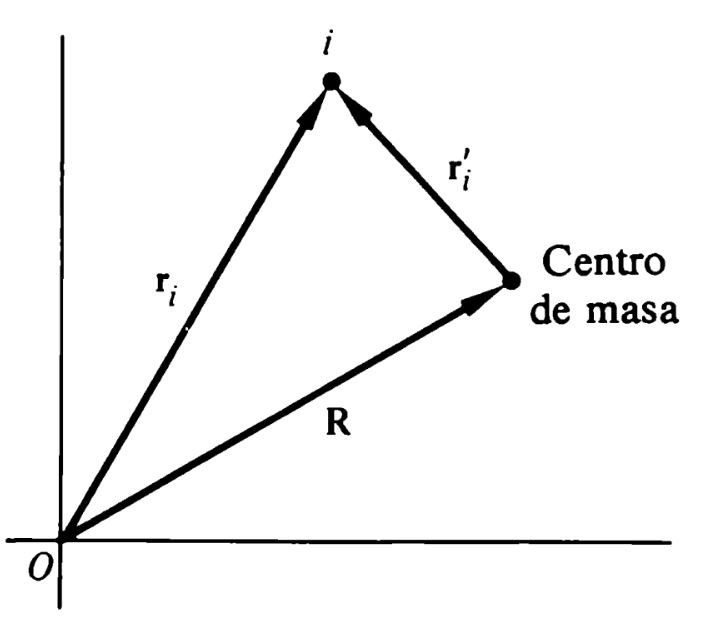
\includegraphics[scale=0.4]{images/cm.JPG}
        \caption{Vectores que intervienen en el cambio de punto de referencia para el momento cinético}
        \label{fig:fig1}
    \end{figure}
    \vspace{0.2cm}

Por ultimo, consideraremos la ecuación de la energía. Al igual que en el caso de la partícula, calculamos el trabajo efectuado por todas las fuerzas al mover el sistema de una configuración inicial $1$ a una configuración final $2$:
    
    \begin{equation}
        W_{12}=\sum_i \int_1^2 \vec{F}_i \cdot \text{d} s_i=\sum_i \int_1^2 \vec{F}_i^{(e)}\cdot \text{d}s_i+\underset{i \neq j}{\sum_{i,j}} \int_1^2 \vec{F}_{ji} \cdot \text{d} s_i
        \label{eq28}
    \end{equation}
Utilizando las ecuaciones de movimiento las integrales se reducen a:
    \begin{equation*}
        \sum_i \int_1^2 \vec{F}_i \cdot \text{d} s_i=\sum_i \int_1^2 m_i \dot{\vec{v}}_i \cdot \vec{v}_i \text{d} t= \sum_i \int_1^2 \text{d} \left( \dfrac{1}{2}m_i \vec{v}_i^2 \right)
    \end{equation*}
Sabiendo que el trabajo sigue pudiéndose representar en forma de la variación de la energía cinética:
    \begin{equation*}
        W_{12}=T_2-T_1
    \end{equation*}
Donde la energía cinética total del sistema esta definida como:
    \begin{equation}
        T=\dfrac{1}{2}\sum_i m_i \vec{v}_i^2
        \label{eq29}
    \end{equation}
Si utilizamos las transformaciones a las coordenadas del centro de masa vistas anteriormente en la ecuación \eqref{eq25} y \eqref{eq26}, también podemos expresar la energía cinética de la forma:
    \begin{align*}
        T&=\dfrac{1}{2} \sum_i m_i \vec{v}_i^2 \\
        &=\dfrac{1}{2} \sum_i m_i (\vec{v}+\vec{v}_i^{'})\cdot (\vec{v}+\vec{v}_i^{'}) \\
        &=\dfrac{1}{2} \sum_i m_i v^2+\dfrac{1}{2} \sum_i m_i v'_i^2+\vec{v}\cdot\dfrac{\text{d}}{\text{d}t}  \cancelto{0}{\left( \sum_i m_i \vec{r}_i^{'}\right)} 
    \end{align*}
quedándonos la energía cinética de la forma:
\begin{equation}
    T=\dfrac{1}{2} M v^2+\dfrac{1}{2}\sum_i m_i v' _i^2
    \label{eq30}
\end{equation}
De la ecuación \eqref{eq30} nos damos cuenta que la energía cinética consta de dos partes; la energía cinética que es obtenida considerando toda la masa concentrada en el centro de masa y también la energía cinética del movimiento alrededor del centro de masa.
\\
\vspace{0.2cm}

Ahora si consideramos el segundo miembro de la ecuación \eqref{eq28}. En el caso particular de que las fuerzas exteriores deriven de un potencial, el primer termino lo podremos escribir de la siguiente manera:
\begin{equation*}
    \sum_i \int_1^2 \vec{F}_i^{(e)} \cdot \text{d} s_i= -\sum_i \int_1^2 \nabla_i V_i \cdot ds_i= -  \left \sum_i V_i \right |_1^2
\end{equation*}
donde el subíndice $i$ del operador nos indica que las derivadas se realizaran respecto alas componentes $\vec{r}_i$. Las fuerzas mutuas entre las partículas $i$-ésima y $j$-ésima $\vec{F}_{ij}$ y $\vec{F}_{ji}$ podrán obtenerse a partir de una función potencial $V_{ij}$, de la forma:
\begin{equation}
    V_{ij}=V_{ij} (|\vec{r}_i-\vec{r}_j|)
    \label{eq31}
\end{equation}
Si las dos fuerzas son iguales y opuestas:
\begin{equation}
    \vec{F}_{ij}=-\nabla_i V_ij=+\nabla_j V_{ij}=-\vec{F}_{ij}
    \label{eq32}
\end{equation}
y las cuales están soportadas por la recta que une ambas partículas de la forma:
\begin{equation}
    \nabla V_{ij} (|\vec{r}_i-\vec{r}_j|)=(\vec{r}_i-\vec{r}_j) f
    \label{eq33}
\end{equation}
donde $f$ es una cierta función escalar.

\vspace{0.2cm}
Cuando las fuerzas sean todas conservativas se podrá escribir el ultimo termino de la ecuación \eqref{eq28} de la forma:

\begin{equation}
    W_{12}=-\sum_i \int_1^2 \nabla_i V_i \cdot \text{d} \vec{s_i}-\dfrac{1}{2} \underset{i \neq j}{\sum_i \sum_j} \nabla V_{ij} V_{ij} \cdot \text{d} \vec{r}_{ij}
    \label{eq34}
\end{equation}

El último término se obtiene de escribir $\sum_i \sum_j$ en forma de pares:
\begin{align}
    \int_1^2 \left( \vec{F}_{ji}\cdot \text{d} \vec{s}_i +\vec{F}_{ij} \cdot \text{d} \vec{s}_j \right)=-\int_1^2 \left ( \nabla_i V_{ij} \cdot \text{d} \vec{s}_i+ \nabla_j V_{ij} \cdot \text{d} \vec{s}_j \right)
    \label{eq35}
\end{align}
Si representamos por $\vec{r}_{ij}$ la diferencia de vector $\vec{r}_i-\vec{r}_j$ y si $\nabla_{ij}$ representa el gradiente respecto a $\vec{r}_{ij}$, será:
\begin{equation}
    \nabla_i V_{ij}=\nabla_{ij} V_{ij}= -\nabla_j V_{ij}
    \label{eq36}
\end{equation}
y también
\begin{equation}
    \text{d} \vec{s}_i-\text{d}\vec{s}_j=\text{d} \vec{r}_i-\text{d}\vec{r}_j=\text{d} \vec{r}_{ij}
    \label{eq37}
\end{equation}
De lo cual obtenemos de la ecuación \eqref{eq35}:
\begin{align*}
    \int_1^2 \left( \vec{F}_{ji}\cdot \text{d} \vec{s}_i +\vec{F}_{ij} \cdot \text{d} \vec{s}_j \right)&=-\int_1^2 \left ( \nabla_i V_{ij} \cdot \text{d} \vec{s}_i+ \nabla_j V_{ij} \cdot \text{d} \vec{s}_j \right) \\
     &= -\int_1^2 \nabla_{ij} V_{ij} \cdot (\text{d} \vec{s}_i-\text{d}\vec{s}_j) \\
     &= - \int \nabla_{ij} V_{ij} \cdot \text{d} \vec{r}_{ij}
\end{align*}
De este modo el trabajo total debido a las fuerzas interiores se reduce a la siguiente forma:
\begin{equation}
    W_{12}=-\dfrac{1}{2} \underset{i \neq j}{\sum_{i,j}} \int_1^2 \nabla_{ij} V_{ij} \cdot \text{d}\vec{r}_{ij}=-\dfrac{1}{2}  \left \underset{i \neq j}{\sum_{i,j}} V_{ij} \right |_1^2
    \label{eq38}
\end{equation}
De estas consideraciones podemos definir una \textit{energía potencial total}, $V$ del sistema:
\begin{equation}
    V=\sum_i V_i+\dfrac{1}{2} \underset{i \neq j}{\sum_{i,j}} V_{ij}
    \label{eq39}
\end{equation}
tal que se conserve la energía total $T+V$, donde tenemos que este teorema es análogo al de la conservación para una sola partícula. \\
\vspace{0.2cm}

También podemos hacer mención al termino $\dfrac{1}{2} \underset{i \neq j}{\sum_i \sum_j} V_{ij}$ de la ecuación \eqref{eq39} el cual en general no tiene porque ser nulo, ya que puede variar cuando el sistema varía con el tiempo. En los cuerpos rígidos será siempre constante ya que los $\vec{r}_{ij}$ son fijos y no varían con el tiempo de modo que los $\text{d}\vec{r}_{ij}$ solo pueden ser perpendiculares a las $\vec{r}_{ij}$ correspondientes y por tanto a las $\vec{F}_{ij}$ de modo que las fuerzas interiores no trabajan y el potencial interno se mantiene constante y podría no tomarse en cuenta al ser una constante aditiva que puede quitarse según elijamos la referencia nula del potencial.

\section{Ligaduras}

Las ligaduras son restricciones que se tienen sobre las coordenadas de un sistema, y estas se expresan mediante ecuaciones denominadas \textit{ecuaciones de ligadura}.

    \begin{figure}[h]
        \centering
        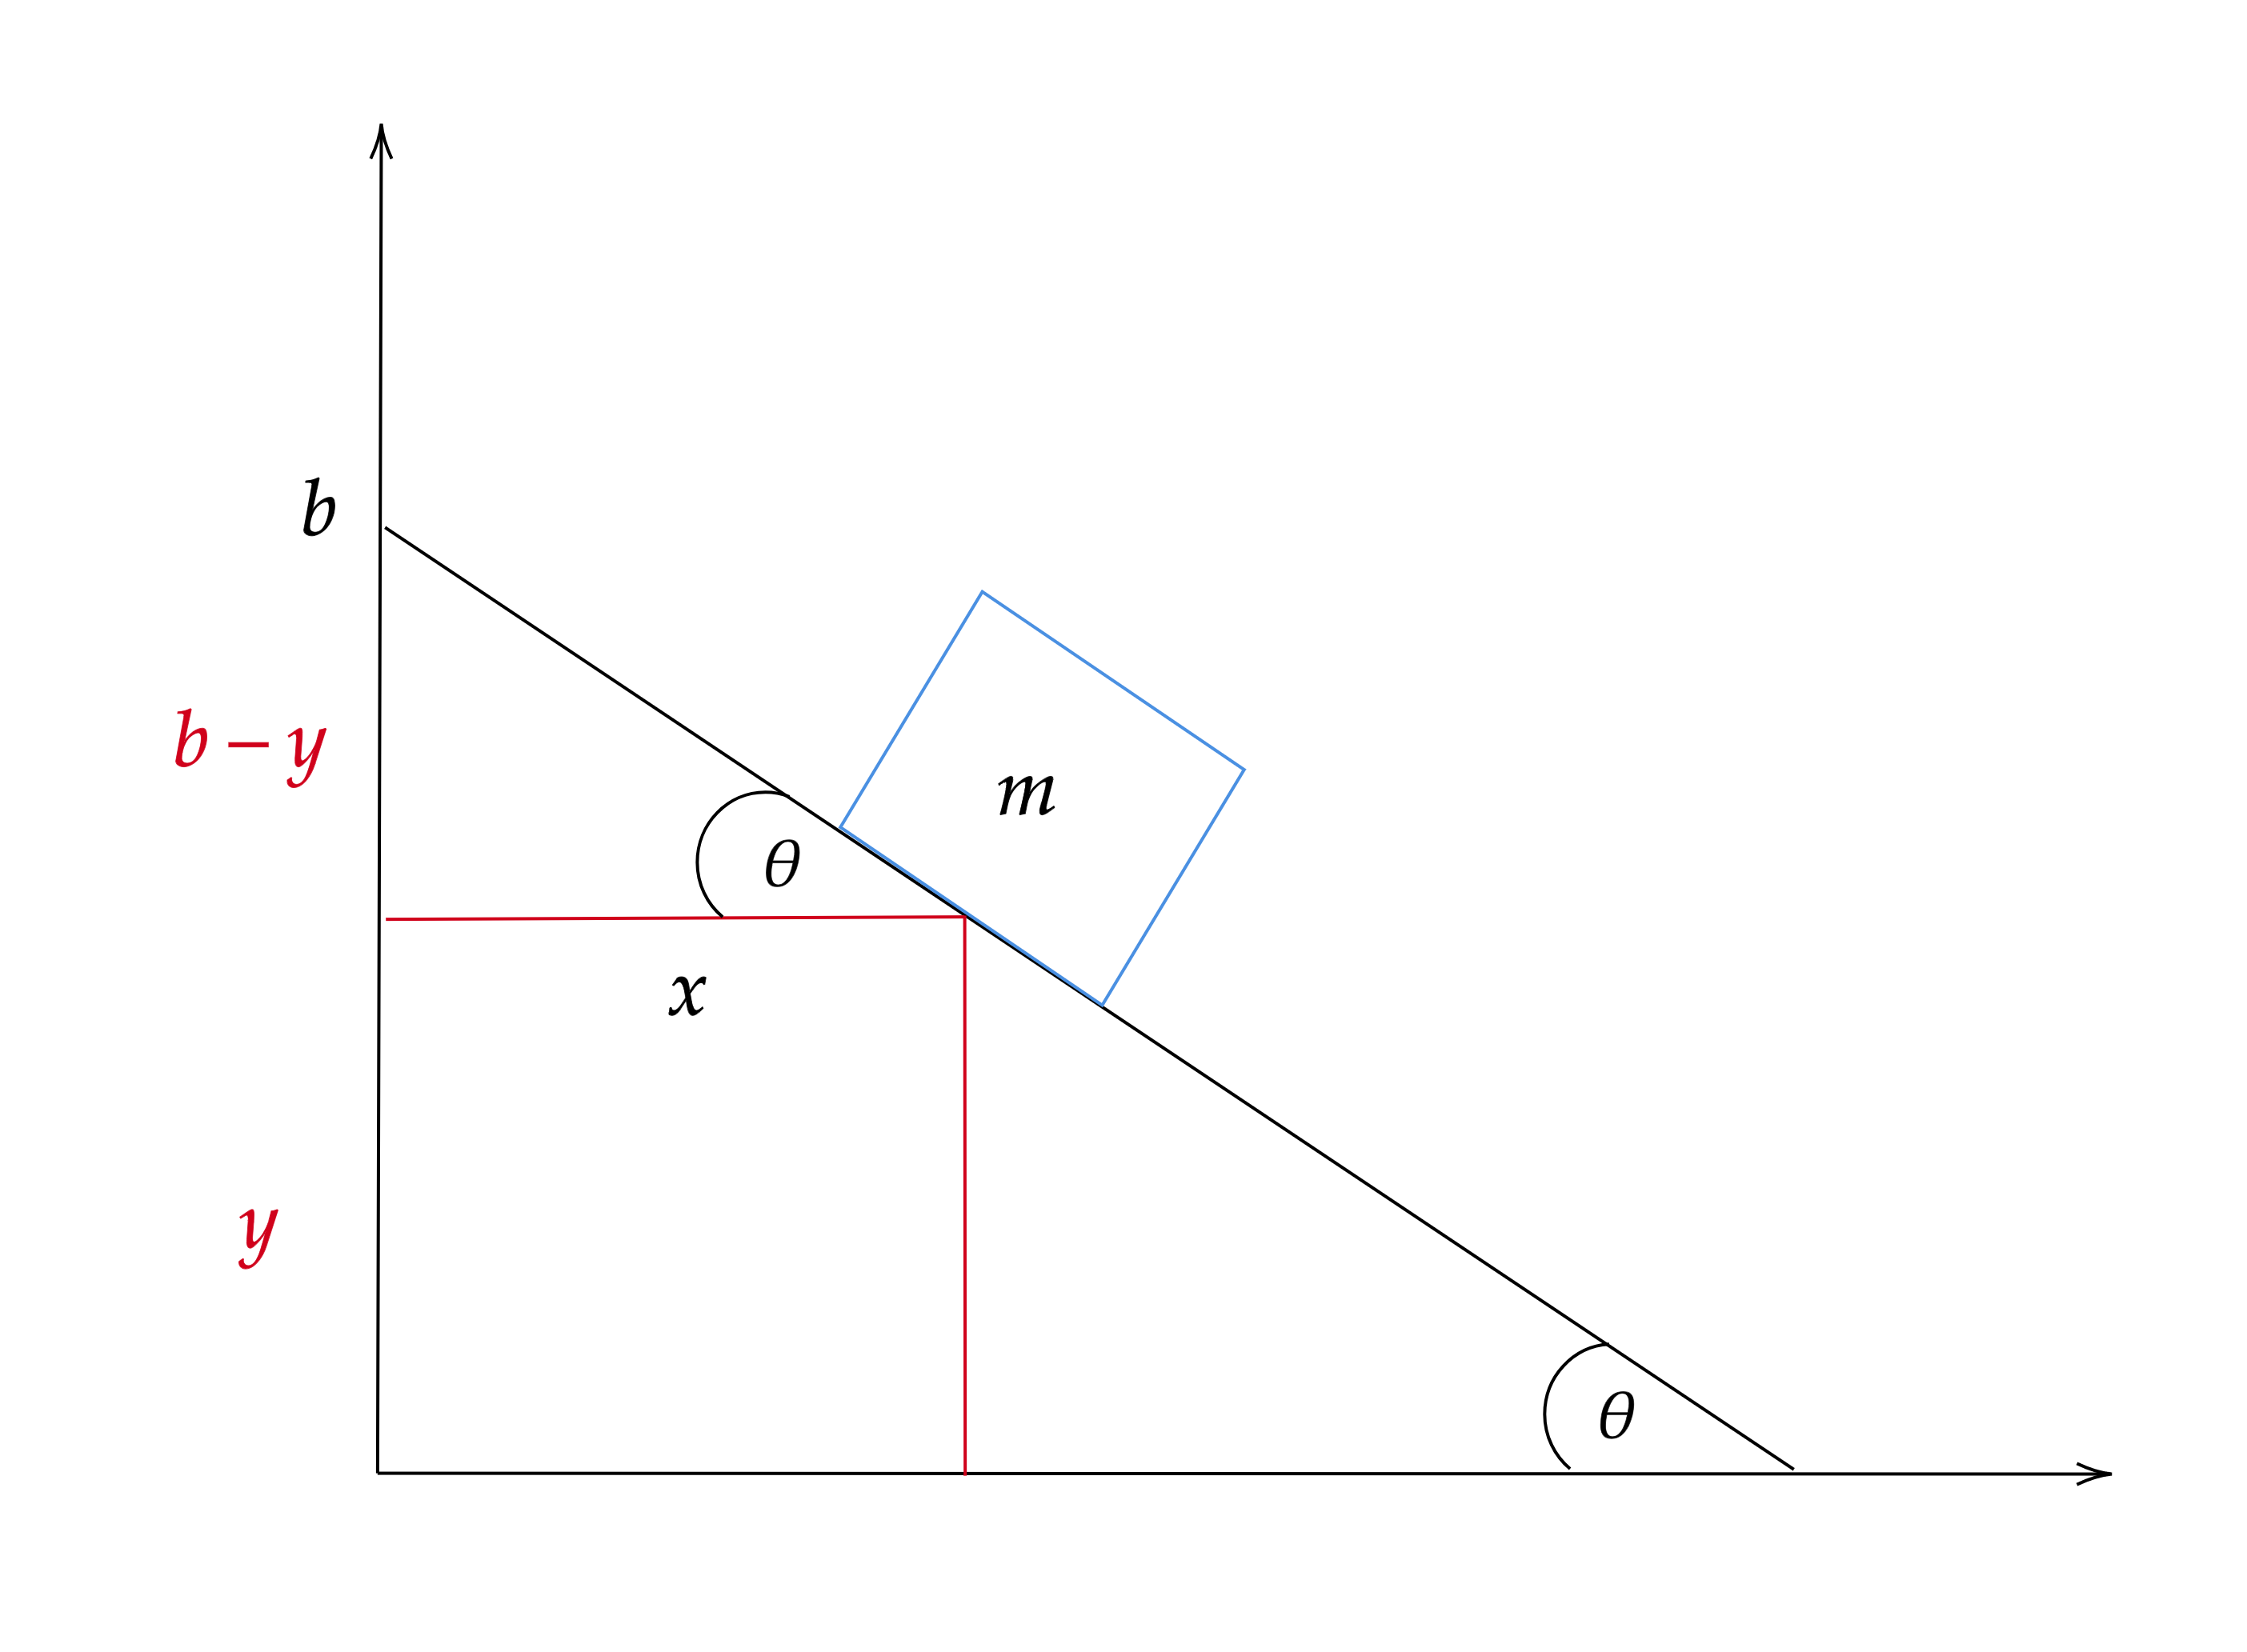
\includegraphics[scale=0.1]{Física Clásica/MECA 2/images/lig1.png}
        \label{fig:fig2}
    \end{figure}
    De la figura tenemos que:
    \begin{align}
        \tan{\theta}=\dfrac{b-y}{x} \quad \righarrow \quad y=-x \tan{\theta}+b
        \label{eq40}
    \end{align}
\subsection*{Ligadura unilateral} 
Este tipo de ligadura se expresa mediante una desigualdad.

    \begin{figure}[h]
        \centering
        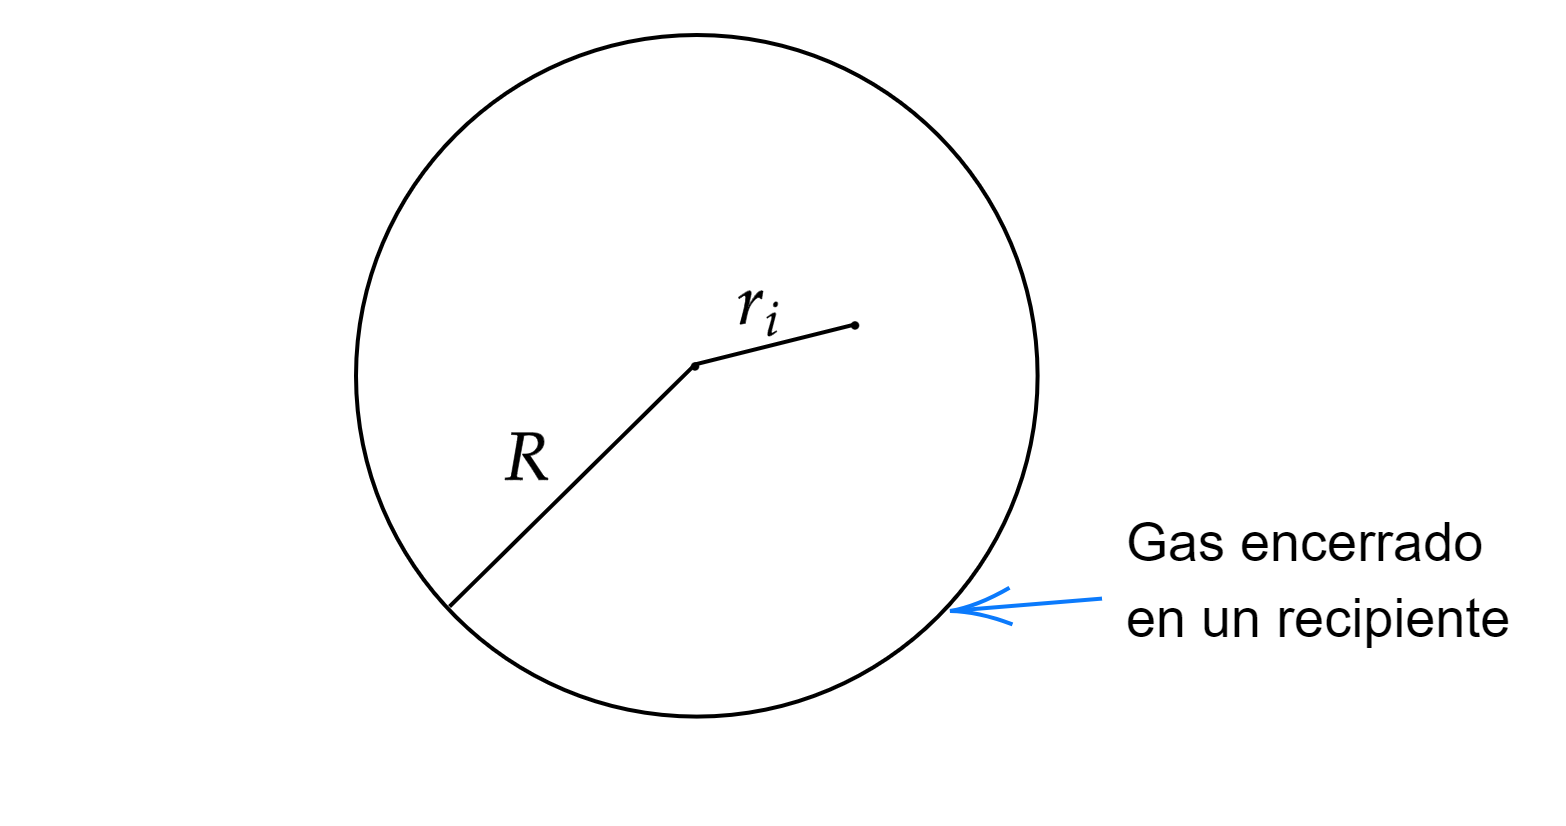
\includegraphics[width=0.6\textwidth]{Física Clásica/MECA 2/images/lig2.png}
        \label{fig:fig3}
    \end{figure}
    Si tenemos que: 
    \begin{align}
        f(\vec{r}_i, \dot{\vec{r}}_i, \cdots, t) \geq 0 \quad ; \quad i=1,2,\cdots,N 
    \end{align}
    Y de la figura se cumple la siguiente desigualdad:
    \begin{align}
        R&-r_i \geq 0
    \end{align}
\subsection*{Ligadura Bilateral}
Esta ligadura a diferencia de la anterior se expresa mediante igualdades de la siguiente forma:

\begin{align}
    f(\vec{r}_i, \dot{\vec{r}}_i, \cdots, t) = 0 \quad \forall \ i
\end{align}

\subsection*{Ligaduras Reónomas}

Estas ligaduras dependen explícitamente del tiempo, por lo cual se denominan ligaduras móviles o cinemáticas.

    \begin{figure}[h]
        \centering
        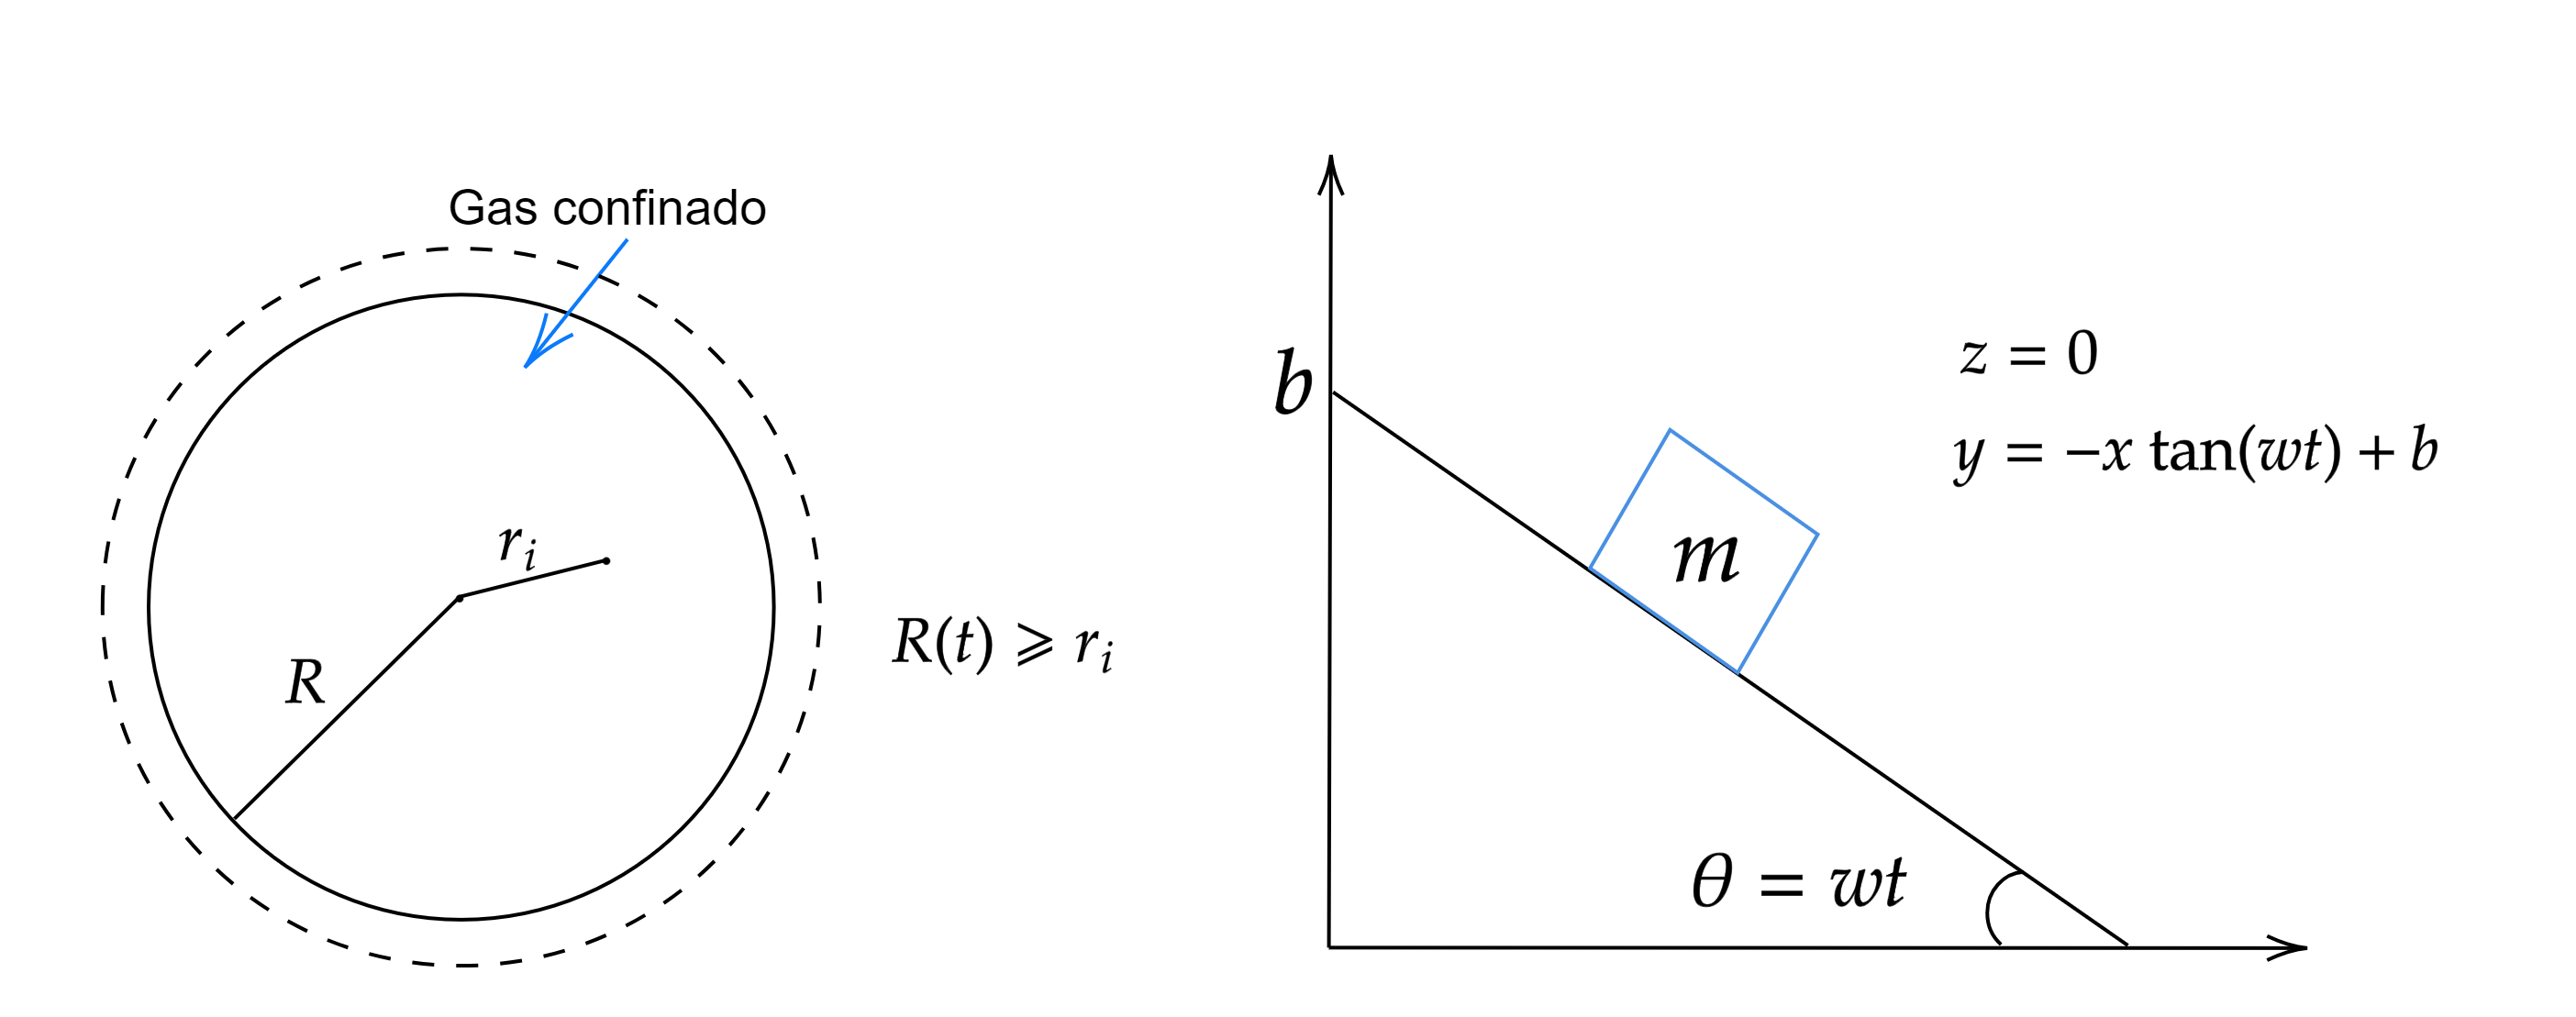
\includegraphics[scale=0.15]{Física Clásica/MECA 2/images/lig3.png}
        \label{fig:fig4}
    \end{figure}

\subsection*{Ligaduras Escleronomas}

Estas ligaduras no dependen explicitamente del tiempo. Y son denominadas fijas o estacionarias.

    \begin{figure}
        \centering
        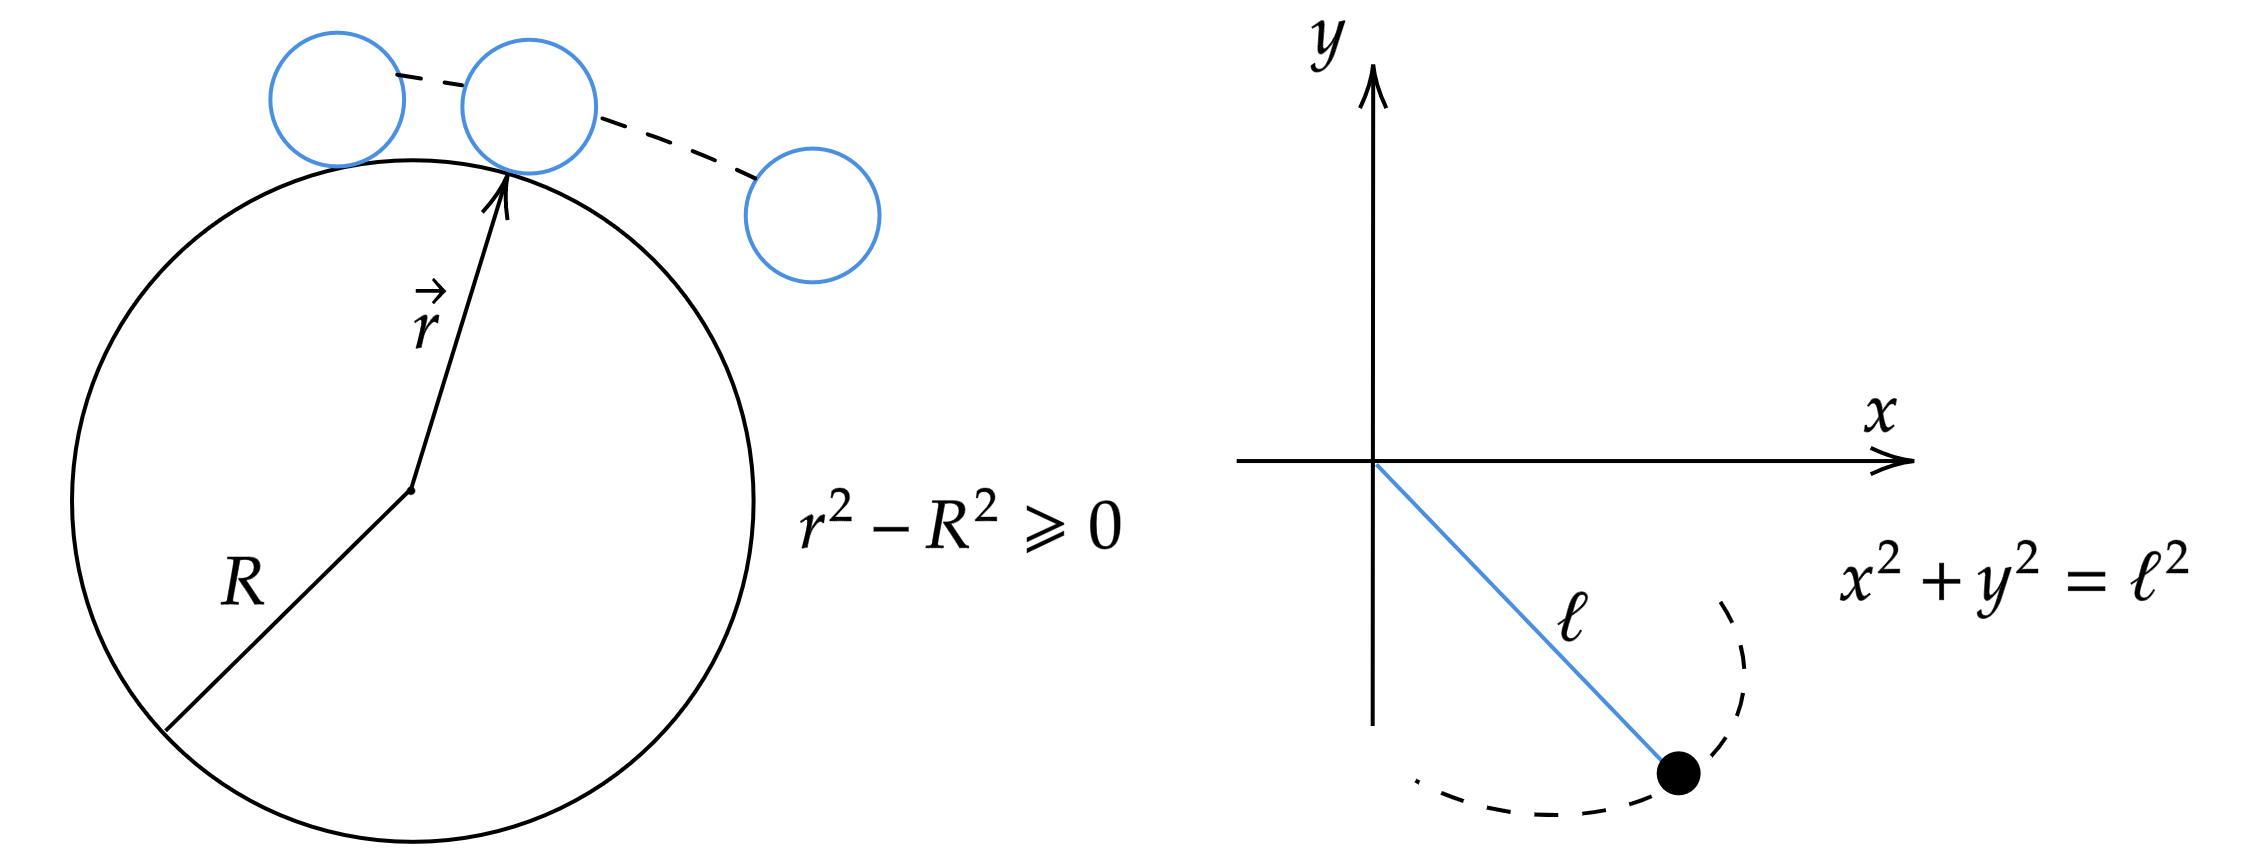
\includegraphics[scale=0.22]{Física Clásica/MECA 2/images/lig4.png}
        \label{fig:fig5}
    \end{figure}
    
\subsection*{Ligaduras Holónomas}
Son aquellas ligaduras bilaterales las cuales no dependen de velocidades pero si dependen exclusivamente de dos cosas:
\begin{align*}
    &\text{- Coordenadas(escleronomas)} \quad \rightarrow \quad f_{\ell}^h(\vec{r}_i,t)=0 \\
    &\text{- Tiempo(Reonomas)} \qquad \qquad \qquad \quad i=1,2,\cdots, N \ ; \ \ell =1,2,\cdots,N
\end{align*}
Estas ligaduras también son llamadas \textit{ligaduras geométricas}. Y un sistema se denominara holónomo cuando todas sus ligaduras sean holónomas.

\subsection*{Grados de libertad configuracionales}

Es el número de coordenadas independientes que junto con las ecuaciones de ligaduras permiten especificar la configuración del sistema.

\begin{equation}
    \underbrace{S=3N-K}_{\text{Grados de libertad configuracionales}}
    \label{eq44}
\end{equation}

\textbf{Ejemplo 1:} Partícula moviendose en entre dos planos

\begin{figure}[h]
    \centering
    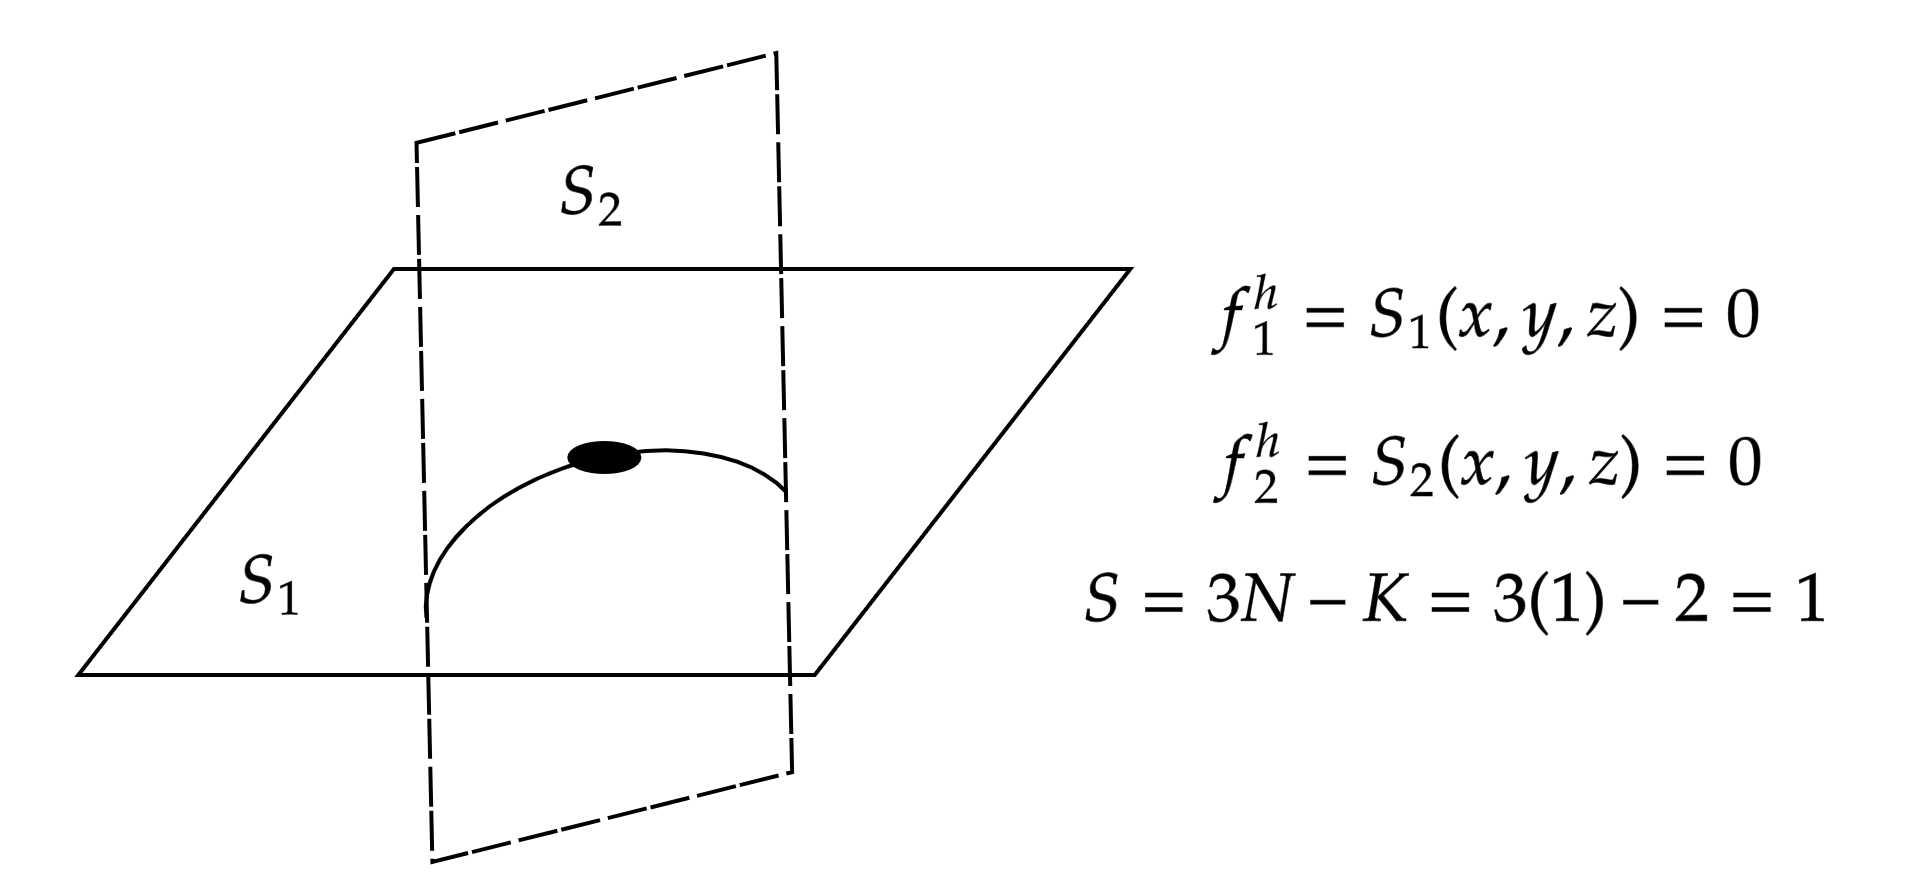
\includegraphics[scale=0.213]{Física Clásica/MECA 2/images/lig6.png}
    \label{fig:fig6}
\end{figure}

\section{Coordenadas Generalizadas}
Se denominan coordenadas generalizadas a un conjunto cualquiera de parámetros $\{ q_i, i=1,2,\cdots,n\}$ que sirven para determinar de manera univoca la configuración del sistema.

El número $n$ de coordenadas generalizadas es el número de grados de libertad.

\subsection*{Ecuaciones de Transformación}

Sea 

\begin{equation}
    \vec{r}_{\gamma} = x_{\gamma}\hat{i}+y_{\gamma}\hat{j}+z_{\gamma}\hat{k}
    \label{eq45}
\end{equation}

la posición de la $\gamma$-ésima partícula. Las coordenadas de posición generalizadas están dadas por:

\begin{align}
    x_{\gamma}&=x_{\gamma}(q_1,q_2,\cdots,q_n,t)=x_{\gamma}(q_i,t) \nonumber \\
    y_{\gamma}&=y_{\gamma}(q_1,q_2,\cdots,q_n,t)=y_{\gamma}(q_i,t) \\
    z_{\gamma}&=z_{\gamma}(q_1,q_2,\cdots,q_n,t)=z_{\gamma}(q_i,t) \nonumber \\
    \vec{r}_{\gamma}&=\vec{r}_{\gamma}(q_1,q_2,\cdots,q_n,t)=\vec{r}_{\gamma}(q_i,t) \nonumber
    \label{eq46}
\end{align}

Y de manera general tenemos:
\begin{equation}
    \vec{r}_i=\vec{r}_i(q_j,t) \left \{ \begin{array}{lcc}
             (i=1,2,\cdots, N)  \\
             \\ (j=1,2,\cdots, N)   
             \end{array} \right.  
             \label{eq47}
\end{equation}
  
También tenemos que:

\begin{equation}
    q_j=q_j(\vec{r}_i,t) \left \{ \begin{array}{lcc}
             (i=1,2,\cdots, N)  \\
             \\ (j=1,2,\cdots, N)   
             \end{array} \right.
             \label{eq48}
\end{equation}

\subsection*{Espacio de Configuraciones}
Es un espacio abstracto constituido por cualquier conjunto de $n$ coordenadas generalizadas $q_i$.

\subsection*{Magnitudes en coordenadas generalizadas}

\begin{enumerate}
    \item DESPLAZAMIENTO
    $$
    d\vec{r}_i=\sum_{j=1}^n \pdv{\vec{r}_i}{q_j}dq_j+\pdv{\vec{r}_i}{t}dt \left \{ \begin{array}{lcc}
             (i=1,2,\cdots, N)  \\
             \\ (j=1,2,\cdots, N)   
    \end{array} \right.
    $$
    \item VELOCIDAD
    $$
    \dot{\vec{r}}_i=\dv{\vec{r}_i}{t}=\sum_{j=1}^n \pdv{\vec{r}_i}{q_j} \dot{q}_j+\pdv{\vec{r}_i}{t}
    $$
    \item ACELERACIÓN
    $$
    \ddot{\vec{r}}_i=\sum_{j=1}^n \dv{}{t}\left( \pdv{\vec{r}_i}{q_j}\dot{q}_j\right)+\dv{}{t}\left( \pdv{\vec{r}_i}{t}\right) 
    $$
    Donde tenemos que:
    \begin{align*}
        \dv{}{t} \left( \pdv{\vec{r}_i}{q_j}\right)&=\sum_{k=1}^n \pdv{^2 \vec{r}_i}{q_k \partial q_j} \dot{q}_k \\
        \dv{}{t} \left( \pdv{\vec{r}_i}{t}\right)&=\sum_{k=1}^n \pdv{^2 \vec{r}_i}{q_k \partial t} \dot{q}_k
    \end{align*}
    Si reemplazamos nos queda:
    $$
    \ddot{\vec{r}}_i=\sum_{j,k}^n \pdv{^2 \vec{r}_i}{q_k \partial q_j} \dot{q}_k \dot{q}_j+\sum_{j=1}^n \left ( \pdv{\vec{r}_i}{q_j}\ddot{q}_j+\pdv{^2 \vec{r}_i}{q_j \partial t} \dot{q}_j \right)
    $$
    \item TRABAJO MECÁNICO
    \begin{align*}
        dW&=\sum_{i=1}^N \vec{F}_i \cdot d\vec{r}_i= \sum_{i=1}^N \vec{F}_i \cdot \left( \sum_{j=1}^n \pdv{\vec{r}_i}{q_j}dq_j+ \pdv{\vec{r}_i}{t}\cdot dt \right) \\
        dW&=\sum_{j=1}^n \underbrace{\left( \sum_{i=1}^N \vec{F}_i \cdot \pdv{\vec{r}_i}{q_j}
     \right)}_{Q_j}dq_j+\sum_{i=1}^N \vec{F}_i \cdot \pdv{\vec{r}_i}{t}dt \\
        dW&=\sum_{j=1}^n Q_j dq_j+\sum_{i=1}^N \vec{F}_i \cdot \pdv{\vec{r}_i}{t}dt
    \end{align*}
    donde: \footnote{La fuerza generalizada no necesariamente tiene dimensión de fuerza.}
    $$
    \underbrace{Q_j=\sum_{i=1}^N \vec{F}_i \cdot \pdv{\vec{r}_i}{q_j} \ ; \ j=1,2,\cdots,n}_{\text{Fuerza Generalizada}}
    $$ 
\end{enumerate}

Notamos que:


\begin{itemize}
    \item Si $q_j$ es longitud $\rightarrow$ $Q_j$ es fuerza.
    \item Si $q_j$ es ángulo $\rightarrow$ $Q_j$ es torque.
    \item Si $q_j$ es superficie $\rightarrow$ $Q_j$ es tensión.
    \item Si $q_j$ es volumen $\rightarrow$ $Q_j$ es presión.
    \item Sin embargo $Q_jdq_j$ $\rightarrow$ siempre tiene dimensión de trabajo.
\end{itemize}

\subsection*{Ejemplos}
\begin{enumerate}
    \item Cilindro rodando sin deslizar

    \noindent\begin{minipage}{.45\textwidth}
  \centering
  \rule{4cm}{3cm}
  \captionof{figure}{Imagen temporal}
  \label{fig:figure}
    \end{minipage}
    \begin{minipage}{.45\textwidth}
    $x$ y $\phi$ son independientes, de modo que:
    
    \begin{align*}
        \dot{x}=R \dot{\phi} \rightarrow \dot{x}-R \dot{\phi}=0 \\
        f(\vec{r}_i,\dot{\vec{r}}_i,t)=0
    \end{align*}
    \end{minipage}
    
    \item Disco vertical rodando sin deslizar

    \noindent\begin{minipage}{.45\textwidth}
  \centering
  \rule{4cm}{3cm}
  \captionof{figure}{Imagen temporal}
  \label{fig:figure}
    \end{minipage}
    \begin{minipage}{.45\textwidth}
    Condición de Rodamiento
    $$
    v=R \dot{\phi}
    $$
    $(x,y)$ coordenadas del centro del disco
    \end{minipage}
\end{enumerate}


\end{document}